\documentclass[tikz,border=0pt]{standalone}
\usepackage[T1]{fontenc}
\usepackage{helvet}
\renewcommand{\familydefault}{\sfdefault}
% Reuse accepted label-free artwork through vector viewports; no pixel editing.
\usepackage{graphicx}
\usetikzlibrary{arrows.meta,calc}
\tikzset{flow/.style={-{Stealth[length=1.6mm,width=1.1mm]},line width=.5pt},
 every node/.style={font=\fontsize{9}{11}\selectfont,align=center,inner sep=1pt}}
% Arguments: source left/top/right/bottom pixels; destination left/bottom/width mm.
\newcommand{\artpiece}[7]{
 \pgfmathsetmacro{\pieceScale}{#7/((#3-#1)*.1)}
 \begin{scope}[shift={(#5,#6)},scale=\pieceScale,transform shape]
  \clip (0,0) rectangle ({(#3-#1)*.1},{(#4-#2)*.1});
  \node[anchor=south west,inner sep=0pt] at ({-#1*.1},{-(931-#4)*.1})
   {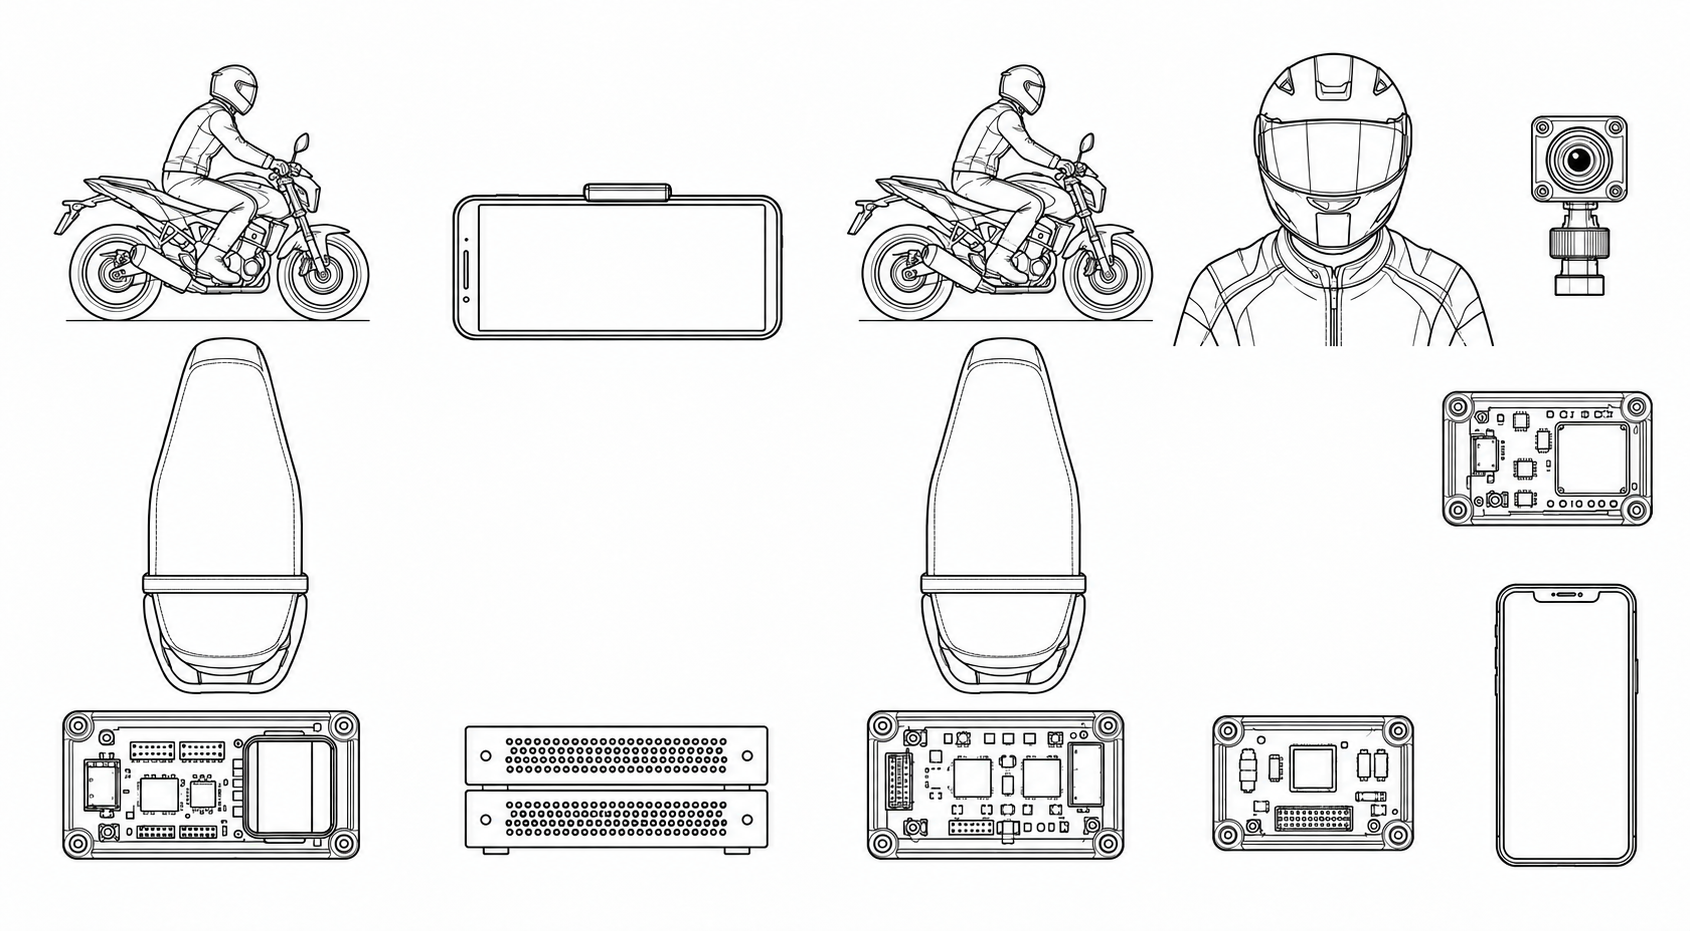
\includegraphics[width=169mm]{../reride/artwork-original.png}};
 \end{scope}}
\newcommand{\marker}[2]{
 \fill[white] (#1-2.4,#2-2.4) rectangle (#1+2.4,#2+2.4);
 \fill (#1-2,#2-2) rectangle (#1+2,#2+2);
 \fill[white] (#1-1.2,#2-1.2) rectangle (#1+1.2,#2+1.2);
 \fill (#1-1.2,#2-1.2) rectangle (#1,#2);
 \fill (#1,#2) rectangle (#1+1.2,#2+1.2);
}
\newcommand{\phoneglyph}[2]{
 \begin{scope}[shift={(#1,#2)}]
  \draw[densely dotted] (-8,0)--(8,0) (0,-13)--(0,13);
  \draw (0,10) .. controls (7,12) and (3,4) .. (7,-1)
    .. controls (11,-9) and (-4,-13) .. (-6,-7)
    .. controls (-9,0) and (-6,8) .. (0,10);
 \end{scope}}

\begin{document}
\begin{tikzpicture}[x=1mm,y=1mm,line width=.4pt,line cap=round,line join=round]
\path[use as bounding box] (0,0) rectangle (240,180);
\node at (120,171) {Personal informatics through embodied self-monitoring};
\artpiece{35}{48}{380}{328}{9}{102}{64}
\node at (41,95) {Everyday motorbike commuting};
\node[draw,minimum width=110mm,minimum height=34mm,align=left] (p17) at (173,132)
 {INTERACT 2017\\2 seat sensors + Genuino + Bluetooth\\Live dashboard + remote retrieval};
\node[draw,minimum width=110mm,minimum height=34mm,align=left] (p19) at (173,74)
 {TEI 2019: Bike Area Network (BANk)\\6 pressure sites + 4 body fiducials\\Pi modules + WebSockets + glanceable display};
\draw[flow] (73,122)--(p17.west);
\draw[flow] (73,112)--(90,112)--(90,74)--(p19.west);
\draw[flow] (p17.south)--(p19.north);
\node[anchor=east] at (170,103) {Modular architecture extends earlier platform};
\draw (8,45)--(232,45);
\node at (42,36) {Before};\node at (120,36) {During};\node at (198,36) {After};
\node at (42,26) {Prepare to ride};\node at (120,26) {Sense + glance};\node at (198,26) {Retrieve + reflect};
\draw[flow] (66,31)--(94,31);\draw[flow] (145,31)--(174,31);
\node at (120,11) {2017: implemented demonstration. 2019: architecture and modules; integrated evaluation remains future work};
\end{tikzpicture}
\end{document}
